\documentclass[12pt,a4paper,twoside,spanish]{article}      % Libro a 11 pt
\usepackage[height=17.5cm,width=13.5cm]{geometry}
\usepackage[english]{babel}         % diccionario
\usepackage[latin1]{inputenc}       % Acentos espa�oles
\usepackage{indentfirst}        % Siempre sangra
\usepackage{fancybox}           % graficos de cajas
\usepackage{epsfig}         % Graficos Postscript
\usepackage{tabularx}
\usepackage{sectsty}
\usepackage{amsmath}        %librer�a de funciones matem�ticas
\usepackage{float}
\usepackage{longtable}
\usepackage{eurosym}
\usepackage{etoolbox,refcount}
\usepackage{multicol}
\usepackage{fancyhdr} 
\usepackage[dvipsnames]{xcolor}
\usepackage[hidelinks]{hyperref}
\graphicspath{{figures/}}

%%%%%%%%%%%%%%%%%%%%%%%%%%%%%%%%%%%%%%%%%%%%%%%
%%%%%%%%%%%%%
%%%%%%%%%%%%% Margenes
%%%%%%%%%%%%%
%%%%%%%%%%%%%%%%%%%%%%%%%%%%%%%%%%%%%%%%%%%%%%%
%%%%% Definimos el maximo tama�o posible.
\marginparwidth 0pt     \marginparsep 0pt
\topmargin   0pt        \textwidth   6.5in
\textheight 23cm

% Margen izq del txt en impares.
\setlength{\oddsidemargin}{.0001\textwidth}

% Margen izq del txt en pares.
\setlength{\evensidemargin}{-.04\textwidth}

% Anchura del texto
\setlength{\textwidth}{.99\textwidth}


%%%%%%%%%%%%%%%%%%%%%%%%%%%%%%%%%%%%%%%%%%%%%%%
%%%%%%%%%%%%%
%%%%%%%%%%%%% Profundidad de enumeracion y tabla de contenidos
%%%%%%%%%%%%%
%%%%%%%%%%%%%%%%%%%%%%%%%%%%%%%%%%%%%%%%%%%%%%%

\setcounter{secnumdepth}{4}
\setcounter{tocdepth}{4}


%%%%%%%%%%%%%%%%%%%%%%%%%%%%%%%%%%%%%%%%%%%%%%%
%%%%%%%%%%%%%
%%%%%%%%%%%%% Nuevos Comandos
%%%%%%%%%%%%%
%%%%%%%%%%%%%%%%%%%%%%%%%%%%%%%%%%%%%%%%%%%%%%%

            %%%%%%%%%%%%%%%%%%%%%%%
            %%%%%%%%%%%%%%%%%%%%%%%
            % Comandos para simplificar
            % la escritura
            %%%%%%%%%%%%%%%%%%%%%%%
            %%%%%%%%%%%%%%%%%%%%%%%

\def\mc{\multicolumn}
            %%%%%%%%%%%%%%%%%%%%%%%
            % Comandos para poder utilizar raggedright en tablas
            %%%%%%%%%%%%%%%%%%%%%%%
\newcommand{\PreserveBackslash}[1]{\let\temp=\\#1\let\\=\temp}
\let\PBS=\PreserveBackslash


%https://tex.stackexchange.com/questions/194426/split-itemize-into-multiple-columns

\newcounter{countitems}
\newcounter{nextitemizecount}
\newcommand{\setupcountitems}{%
	\stepcounter{nextitemizecount}%
	\setcounter{countitems}{0}%
	\preto\item{\stepcounter{countitems}}%
}
\makeatletter
\newcommand{\computecountitems}{%
	\edef\@currentlabel{\number\c@countitems}%
	\label{countitems@\number\numexpr\value{nextitemizecount}-1\relax}%
}
\newcommand{\nextitemizecount}{%
	\getrefnumber{countitems@\number\c@nextitemizecount}%
}
\newcommand{\previtemizecount}{%
	\getrefnumber{countitems@\number\numexpr\value{nextitemizecount}-1\relax}%
}
\makeatother    
\newenvironment{AutoMultiColItemize}{%
	\ifnumcomp{\nextitemizecount}{>}{3}{\begin{multicols}{2}}{}%
		\setupcountitems\begin{itemize}}%
		{\end{itemize}%
		\unskip\computecountitems\ifnumcomp{\previtemizecount}{>}{3}{\end{multicols}}{}}

%%%%%%%%%%%%%%%%%%%%%%%%%%%%%%%%%%%%%%%%%%%%%%%
%%%%%%%%%%%%%
%%%%%%%%%%%%% Cuerpo del documento
%%%%%%%%%%%%%
%%%%%%%%%%%%%%%%%%%%%%%%%%%%%%%%%%%%%%%%%%%%%%%


\begin{document}
\setlength{\parindent}{0pt}
\def\chaptername{Chapter}
\def\tablename{Table}
\renewcommand\listtablename{Index}
\renewcommand\contentsname{Index}
\chapterfont{\LARGE\raggedleft}

\hypersetup{
	linkcolor=black,
	urlcolor=black
}
%%%%%%%%%%%%%%%%%%%%%%%%%%%%%%%%%%%%%%%%%%%%%%%%%%%%%%%%%%%%%%%
%%%%%%%%%%%%%%%%%%%%%%%%%%%%%%%%%%%%%%%%%%%%%%%%%%%%%%%%%%%%%%%
% DISE�O DE LA PAGINA DEL TITULO
%%%%%%%%%%%%%%%%%%%%%%%%%%%%%%%%%%%%%%%%%%%%%%%%%%%%%%%%%%%%%%%
%%%%%%%%%%%%%%%%%%%%%%%%%%%%%%%%%%%%%%%%%%%%%%%%%%%%%%%%%%%%%%%
\pagestyle{empty}
\begin{titlepage}
\setlength{\parindent}{0cm} \setlength{\parskip}{0cm}

% \raggedleft {\textsf{\textbf{Versi�n: 1}}}


\definecolor{udcpink}{RGB}{210, 0, 123}
\newcommand{\HRule}{\rule{\linewidth}{1mm}}
%color udc 210 0 123
\vspace{-2cm}
\begin{center}
	\centering
	\textcolor{udcpink}{\textbf{Facultade de Inform�tica da Coru�a}}
\end{center}
\vspace*{-1.1cm}

\begin{figure}[htbp]
	\hspace*{-3cm}
	\centering
	
\includegraphics[scale=0.35]{UDC_logo.png}
\end{figure}

\begin{center}
	\centering
	TRABALLO DE FIN DE GRAO\\
	GRAO EN INXENAR�A INFORM�TICA\\
	MENCI�N EN COMPUTACI�N\\
\end{center}

\vspace*{2.5cm}
\HRule \\[0.5cm]
\begin{center}
	% Letra lineal y negrita
	\textsf{\textbf{\Large IMPLEMENTATION OF AN AUTOMATIC CAMERA \\[0.25cm] OPERATOR USING DEEP REINFORCEMENT LEARNING \\[0.5cm]}}
	\HRule \vspace*{3cm}
\end{center}
\vspace*{2.5cm}
\raggedleft
\begin{tabular}{@{}cm{5.5cm}@{}}
		\textbf{Student:} & Rodriguez Louz�n, Adri�n\\
		\textbf{Directors:} & Francisco Javier Taibo Pena \\
		 & Emilio Jos� Padr�n Gonz�lez  \\
		 & Luis Omar �lvarez Mures\\
\end{tabular}

\vspace*{\fill}

A Coru�a 13th November of 2020\\ 
\end{titlepage}



\cleardoublepage


\begin{center}
	\flushright
	\thispagestyle{empty}
	\vspace*{\fill}
	To my family and my brother
	\vspace*{\fill}
\end{center}

\cleardoublepage
\setlength{\parskip}{0,4cm}
\newcommand{\newpara}
{
	\vskip 0.3cm
}
\begin{center}
	\textbf{Acknowledgements}\\
	\flushleft
	First of all, I would like to thank my family for supporting me unconditionally and placing all their trust in me.\\
	\newpara
	Thanks also to my friends, those that I made during this 4 years,
	but even more to those who I met during my internation experience in South Korea.\\
	\newpara
	Finally, I want to give my gratitude to my project managers Francisco Javier Taibo Pena, Emilio Jos� Padr�n Gonzalez and Luis Omar �lvarez Mures, without whom I could not have carried out this project. Thank you for all your attention.
\end{center}
\cleardoublepage


\begin{center}
	\textbf{Abstract}\\
	\flushleft
	\newpara
Reinforcement learning (RL) is an area of machine learning concerned with how software agents ought to take
actions in an environment so as to maximize some notion of cumulative reward. \\ 
\newpara
The problems of interest in reinforcement learning have also been studied in the theory of optimal control,
which is concerned mostly with the existence and characterization of optimal solutions, and algorithms for their
exact computation, and less with learning or approximation, particularly in the absence of a mathematical model
of the environment. Reinforcement algorithms that incorporate deep learning can beat world champions at the
game of Go as well as human experts playing numerous Atari video games.\\
\newpara
In this project, we will leverage Deep Reinforcement Learning and game engines to model a typical sports scene
and teach an agent to capture the action on camera. First, a scene which resembles a sports match will be
created using the chosen game engine. Next, we will test out different Deep Reinforcement Learning algorithms.
\newpara
\end{center}

\begin{center}
	\textbf{Resumen}\\
	\flushleft
\newpara
El aprendizaje por refuerzo (AR) es un �rea del aprendizaje autom�tico que se ocupa de c�mo los agentes software deben tomar acciones en un entorno para maximizar alguna noci�n de recompensa acumulativa. \\
\newpara
Los problemas de inter�s en el aprendizaje por refuerzo tambi�n se han estudiado en la teor�a del control �ptimo,
que se ocupa principalmente de la existencia y caracterizaci�n de soluciones �ptimas y algoritmos para su
c�lculo exacto, y menos con aprendizaje o aproximaci�n, particularmente en ausencia de un modelo matem�tico
del medio ambiente. Los algoritmos de refuerzo que incorporan el aprendizaje profundo pueden vencer a los campeones mundiales en el Juego de Go, as� como expertos humanos que juegan numerosos videojuegos de Atari. \\
\newpara
En este proyecto, aprovecharemos el aprendizaje de refuerzo profundo y los motores de juego para modelar una escena deportiva t�pica y ense�arle a un agente a capturar la acci�n con la c�mara. Primero, una escena que se asemeja a un partido deportivo ser� creado utilizando el motor de juego elegido. A continuaci�n, probaremos diferentes algoritmos de aprendizaje por refuerzo profundo.

\end{center}
\newpage
\begin{center}
\flushleft
\textbf{Keywords}
\begin{AutoMultiColItemize}
	\item Artificial Intelligence
	\item Deep Reinforcement Learning
	\item Camera operator
	\item DQN
	\item Python
	\item Tensorflow
	\item Keras
\end{AutoMultiColItemize}	
\end{center}

\mbox{}
\setcounter{page}{2}






\newpage



%%%%%%%%%%%%%%%%%%%%%%%%%%%%%%%%%%%%%%%%%%%%%%%
%%
%% TABLA DE CONTENIDOS
%%
%%%%%%%%%%%%%%%%%%%%%%%%%%%%%%%%%%%%%%%%%%%%%%%
\tableofcontents
\cleardoublepage


%%%%%%%%%%%%%%%%%%%%%%%%%%%%%%%%%%%%%%%%%%%%%%%%%%%%%%%%%%%%%%%
%%%%%%%%%%%%%%%%%%%%%%%%%%%%%%%%%%%%%%%%%%%%%%%%%%%%%%%%%%%%%%%
%CONTENIDO DEL DOCUMENTO
%%%%%%%%%%%%%%%%%%%%%%%%%%%%%%%%%%%%%%%%%%%%%%%%%%%%%%%%%%%%%%%
%%%%%%%%%%%%%%%%%%%%%%%%%%%%%%%%%%%%%%%%%%%%%%%%%%%%%%%%%%%%%%%

%numeros ar�bigos
%\markboth{Implementation of an automatic camara %operator}{University of A Coru�a.}

%indentaciones y espaciado entre p�rrafos
%\setlength{\parskip}{0,3cm}

\pagestyle{fancy}

\cfoot{\thepage} 
\pagenumbering{arabic}



%%%%%%%%%%%%%%%%%%%%%%%%%%%%%%%%%%%%%%%%%%%%%%%%%%%%%%%%%%%%%%%%%%%%%%%%%%%%%%%
\section{Introduction.}
%%%%%%%%%%%%%%%%%%%%%%%%%%%%%%%%%%%%%%%%%%%%%%%%%%%%%%%%%%%%%%%%%%%%%%%%%%%%%%%
Deep Reinforcement Learning (DRL), a very fast-moving field, is the combination of Reinforcement Learning and Deep Learning and it is also the most trending type of Machine Learning at this moment because it is being able to solve a wide range of complex decision-making tasks that were previously out of reach for a machine to solve real-world problems with human-like intelligence.\\
\newpara
In this introduction I will try to explain the fundamentals and concepts around Artificial intelligence and Machine Learning, in order to then deeply dive into our program and how I implemented it.

%%%%%%%%%%%%%%%%%%%%%%%%%%%%%%%%%%%%%%%%%%%%%%%%%%%%%%%%%%%%%%%%%%%%%%%%%%%%%%%
\subsection{Artificial Intelligence and Machine Learning}
%%%%%%%%%%%%%%%%%%%%%%%%%%%%%%%%%%%%%%%%%%%%%%%%%%%%%%%%%%%%%%%%%%%%%%%%%%%%%%%
We can divide Artificial Intelligence into two categories \textbf{Narrow AI} and \textbf{General A.I.}

\begin{figure}[htbp]
	\centering
	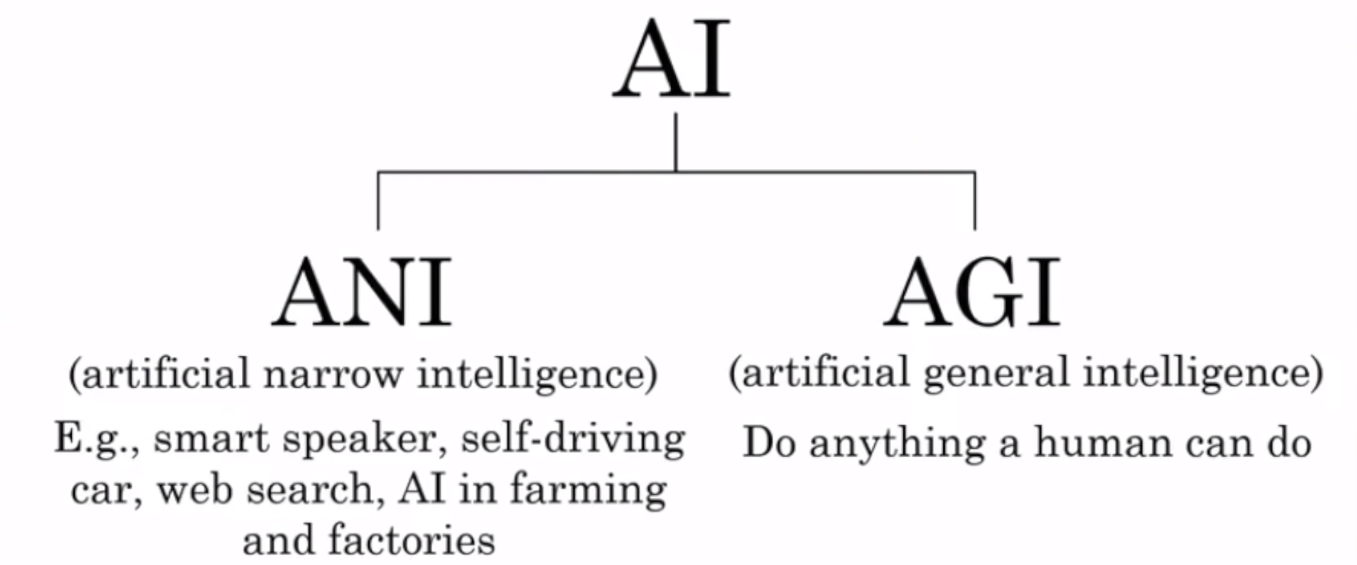
\includegraphics[scale=0.35]{cattegories_AI.png}
	\caption{Categories of Artificial Intelligence}
\end{figure}

Most of the movies and representations that we see in the mainstream media are around General A.I. Machines that do everything that humans do, and better. It can talk, it can learn to play games, it can communicate... etc \\
\newpara
Right now, in our field we are working on narrow A.I. Are machines that can do only one thing and the application of the machine is narrowed to a specific goal. In this field and in the recent years, great advances were made.For instance, AlphaGo defeated the best professional human player in the game of Go. Or last year, for instance, our friend Oriol Vinyals and his team in DeepMind showed the AlphaStar agent beat professional players at the game of StarCraft II. Or a few months later, OpenAI?s Dota-2-playing bot became the first AI system to beat the world champions in an e-sports game.\\
\newpara

Machine Learning ~\cite{ml4dummies} is one of the many approaches that Artificial Intelligence (AI) uses when it comes to extracting knowledge from experience, not only as a tool to
achieve the objectives linked to AI but as a vehicle to reduce time and effort
used for resolution. ML recognizes patterns through the use of examples in
rather than addressing its implementation. The machine learns a model from examples and
use this one to solve the problem. A system that continuously learns, that is capable of
make decisions based on data instead of algorithms and that changes your behavior, it is a system based on ML.
Given a problem the choice of the appropriate algorithm is not trivial. For this it is necessary
ask yourself two fundamental questions: what do I want to do? and what information
I have to achieve my goal? Both require us to carry out an exhaustive analysis of the
own problem and the data, quantity and quality, that we have for its resolution.

\begin{figure}[htbp]
	\centering	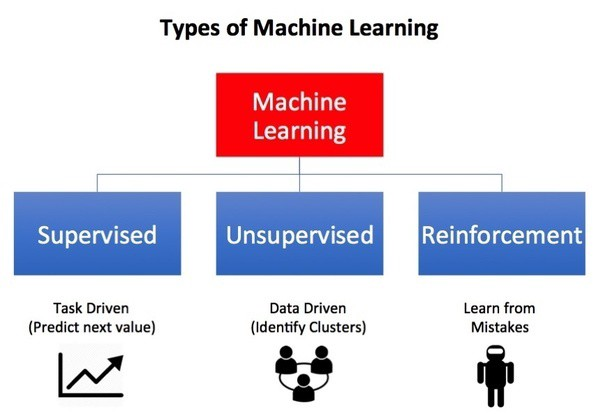
\includegraphics[scale=0.50]{machine_learning.jpeg}
	\caption{Types of Machine Learning}
\end{figure}

Reinforcement Learning is one of the three branches in which ML techniques are generally categorized:

\begin{itemize}
	\item \textbf{Supervised Learning}is the task of learning from tagged data and its goal is to generalize.
	\item \textbf{Unsupervised Learning}is the task of learning from unlabeled data and its goal is to compress.
	\item \textbf{Reinforcement Learning} is the task of learning through trial and error and its goal is to act.
\end{itemize}

Orthogonal to this categorization we can consider a powerful recent approach to ML, called \textbf{Deep Learning (DL)}, topic of which we have discussed extensively in previous posts. DL is not a separate branch of ML, so it?s not a different task than those described above. DL is a collection of techniques and methods for using neural networks to solve ML tasks, either Supervised Learning, Unsupervised Learning, or Reinforcement Learning and we can represent it graphically in the following figure:

\begin{figure}[htbp]
	\centering
	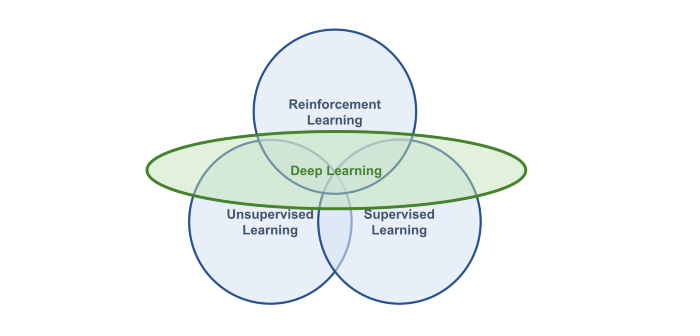
\includegraphics[scale=0.50]{deep_learning.png}
	\caption{Visual relationship of Deep Learning with the Machine Learning categories.}
\end{figure}


Reinforcement learning ~\cite{reinfLearning}~\cite{introReinf} is a form of machine learning in which an agent attempts to
learn a policy that maximizes a numeric reward signal~\cite{introReinf}. In reinforcement learning,
an agent learns by trial and error and discovers optimal actions through its own experiences. Unlike supervised learning, the agent does not learn by comparing its own actions to those of an expert; everything it learns is from its own interactions with the environment. Reinforcement learning attempts to solve optimization problems that are
defined by a Markov Decision Process (MDP) ~\cite{introReinf}. A A Markov Decision Process defines
the behavior of the environment by mathematically defining the environment�s one step dynamics.\\

%%%%%%%%%%%%%%%%%%%%%%%%%%%%%%%%%%%%%%%%%%%%%%%%%%%%%%%%%%%%%%%%%%%%%%%%%%%%%%%
\subsection{Elements in Reinforcement Learning}
%%%%%%%%%%%%%%%%%%%%%%%%%%%%%%%%%%%%%%%%%%%%%%%%%%%%%%%%%%%%%%%%%%%%%%%%%%%%%%%
In Reinforcement Learning there are two core components:
\begin{itemize}
	\item \textbf{An Agent}, that represents the "solution" , which is a computer program with a single role of making decisions (actions) to solve complex decision-making problems under uncertainty.
	\item \textbf{An Enviroment}, that is the representation of a "problem", which is everything that comes after the decision of the Agent. The environment responds with the consequences of those actions which are observations or states and rewards also sometimes called costs.
\end{itemize}



For example, let�s take the game of PacMan where the goal of the agent(PacMan) is to eat the food in the grid while avoiding the ghosts on its way. In this case, the grid world is the interactive environment for the agent where it acts. Agent receives a reward for eating food and punishment if it gets killed by the ghost (loses the game). The states are the location of the agent in the grid world and the total cumulative reward is the agent winning the game.

\begin{figure}[htbp]
	\centering
	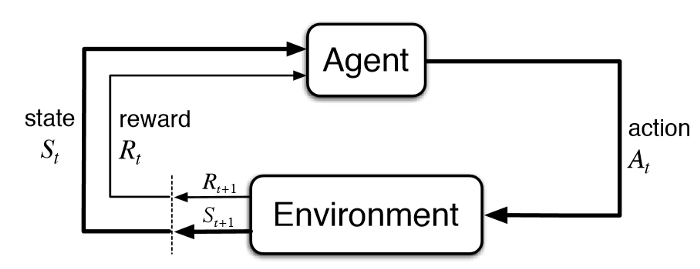
\includegraphics[scale=0.50]{rl_agentenv.png}
	\caption{Reinforcement learning cycle}
\end{figure}
%%%%%%%%%%%%%%%%%%%%%%%%%%%%%%%%%%%%%%%%%%%%%%%%%%%%%%%%%%%%%%%%%%%%%%%%%%%%%%%
\subsection{Q-Learning}
%%%%%%%%%%%%%%%%%%%%%%%%%%%%%%%%%%%%%%%%%%%%%%%%%%%%%%%%%%%%%%%%%%%%%%%%%%%%%%%
Q-Learning is a model-free form of machine learning, in the sense that the AI "agent" does not need to know or have a model of the environment that it will be in. The same algorithm can be used across a variety of environments.

For a given environment, everything is broken down into "states" and "actions." The states are observations and samplings that we pull from the environment, and the actions are the choices the agent has made based on the observation. For the purposes of the rest of this tutorial, we'll use the context of our environment to exemplify how this works.
%%%%%%%%%%%%%%%%%%%%%%%%%%%%%%%%%%%%%%%%%%%%%%%%%%%%%%%%%%%%%%%%%%%%%%%%%%%%%%%
\section{Bibliograf�a}
%%%%%%%%%%%%%%%%%%%%%%%%%%%%%%%%%%%%%%%%%%%%%%%%%%%%%%%%%%%%%%%%%%%%%%%%%%%%%%%
\vspace{-1cm}
\renewcommand\refname{}
\begin{thebibliography}{}
	\bibitem{introReinf} 
	Sutton, R.S. and Barto, A.G. (1998) Reinforcement Learning: An Introduction, Vol. 1. MIT Press, Cambridge. \\
	
	\bibitem{ml4dummies} 
	J. Hurwitz and D. Kirsch, \textit{Machine Learning For Dummies, IBM Limited Edition}, 1st ed.
	John Wiley Sons, Inc., 2018. \\
	
	\bibitem{reinfLearning}
	Kaelbling, L. P., Littman, M. L., Moore, A. W., 1996. Reinforcement learning: A survey. Journal of
	artificial intelligence research 4, 237?285.\\

	
	\bibitem{diegopolo}
	Juan Diego Polo. (2014).
	\textit{ EyeEm compra tecnolog�a para reconocer, clasificar y ordenar fotos. Lugar de publicaci�n: whatsnew.} \\
	\texttt{http://www.hatsnew.com/2014/08/15/eyeem-compra-tecnologia-para-reconocer-\allowbreak clasificar-y-ordenar-fotos/}\\
\end{thebibliography}


%%%%%%%%%%%%%%%%%%%%%%%%%%%%%%%%%%%%%%%%%%%%%%%%%%%%%%%%%%%%%%%
%FINAL DEL LIBRO
%%%%%%%%%%%%%%%%%%%%%%%%%%%%%%%%%%%%%%%%%%%%%%%%%%%%%%%%%%%%%%%
\end{document}
